\section{Сравнение методов рекомендаций рецептов}
Для сравнения рекомендательных алгоритмов выделены следующие критерии:
\begin{itemize}
    \item наличие возможности делать рекомендации для пользователя, если количество оценок от него относительно мало -- К1;
    \item наличие возможности делать рекомендации, если количество пользователей у приложения относительно мало -- К2;
    \item наличие возможности рекомендовать новые рецепты, которые ещё никто не оценил -- К3;
    \item наличие возможности учесть иерархию оценок объекта -- К4;
    \item асимптотика алгоритма -- К5.
\end{itemize}
Критерий <<K1>> необходим для того, чтобы пользователь мог получать рекомендации даже с том случае, если он оценил менее 5 рецептов.
Критерий <<К2>> даёт возможность привлекать пользователей с помощью качественных рекомендаций даже при условии, что их ещё мало.
Таким образом, без удовлетворения критерия <<К2>> приложению будет сложно набрать популярность.
Критерий <<K3>> позволяет добавлять в базу данных новые рецепты, не относящиеся к заранее подготовленному набору данных.
Чтобы сделать оценку пользователя более простой для интерпретации, необходимо дать ему возможность оценивать рецепты по шкале из 5 оценок.
Следовательно, нужно выбрать такой алгоритм рекомендаций, который будет способен работать с не бинарными оценками -- за это отвечает критерий <<К4>>.
Из-за наличия критерия <<К5>> при выборе алгоритма будет учтена его эффективность.
Таким образом, все 5 критериев необходимы для выбора алгоритма рекомендаций.
 
В таблице~\ref{tab:cmp} приведены результаты сравнения всех рассмотренных методов.
Введены следующие обозначения:
\begin{itemize}
    \item $N$ -- количество объектов;
    \item $M$ -- количество параметров объекта;
    \item $U$ -- количество рассматриваемых пользователей;
    \item $S$ -- количество различных дискретных оценок.
\end{itemize}
\begin{table}[h]
\centering
\caption{\centering Сравнение методов по критериям К1--К5}
\begin{tabular}{|l|c|c|c|c|c|c|}
\hline
\textbf{Метод} & \textbf{К1} & \textbf{К2} & \textbf{К3} & \textbf{К4} & \textbf{К5} \\
\hline
Простая коллаборативная фильтрация & -- & -- & + & + & $O(U)$ \\
\hline
Матричные разложения & -- & -- & + & + & $O(U)$ \\
\hline
Гибридная фильтрация & -- & -- & + & + & $O(U+M)$ \\
\hline
Классификация Байеса & -- & + & + & $\pm$ & $O(M)$ \\
\hline
\textit{\textbf{Регрессия}} & -- & + & + & + & $O(M)$ \\
\hline
\textit{\textbf{$k$ ближайших соседей}} & -- & + & + & + & $O(kSM)$ \\
\hline
Комбинация моделей & + & + & + & + & \\
\hline
\end{tabular}
\label{tab:cmp}
\end{table}

На рисунке~\ref{fig:methods} приведена классификация рассмотренных методов.
\begin{figure}[H]
	\centering
	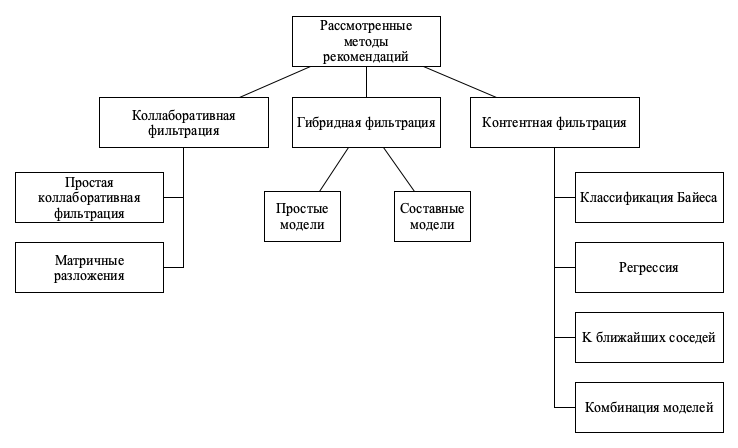
\includegraphics[width=\textwidth]{img/methods.png}
	\caption{
	    Классификация рассмотренных методов рекомендаций
	}
	\label{fig:methods}
\end{figure}
К коллаборативной фильтрации относятся алгоритмы рекомендаций, которые используют оценки данного пользователя и других, но не опираются на содержание рекомендуемых объектов.
Следовательно, если оценок рецептов от различных пользователей недостаточно, то рекомендации будут похожи на случайное угадывание.
Таким образом, данные алгоритмы будут более уместны в том случае, когда приложением пользуется достаточное количество людей, а если у приложения ещё недостаточно пользователей, то следует выбирать другие алгоритмы.
По этой же причине гибридная фильтрация также не выбрана для реализации.

Контентная фильтрация использует данные рекомендуемых объектов и прошлые оценки пользователя.
Поэтому реализация алгоритмов, основанных на ней, требует перевода рецептов в вектора.
Зато при этом отпадает потребность в оценках от разных пользователей.
Классификация Байеса предполагает бинаризацию значений вектора рецепта, вследствие которой часть данных потеряется, и также она хуже работает в случае, когда оценок более двух~\cite{aggarwal}.
Следовательно, её не стоит использовать.
Остальные методы могут быть применены и выбор между ними следует делать в зависимости от точности и эффективности модели рекомендаций.
Таким образом, для реализации выбраны методы <<$k$ ближайших соседей>> и регрессия с уменьшением размерности вектора рецепта.
Это методы с меньшей асимптотикой по сравнению с комбинацией рекомендательных моделей.